\begin{frame}[t]
\frametitle{ChaNGa: Parallel Gravity}
  \begin{itemize}
    \item Collaborative project (NSF)
    \begin{itemize} 
        \item with Tom Quinn, Univ. of Washington
    \end{itemize}
    \pause
    \item Evolution of Universe and Galaxy Formation
    \item Gravity, gas dynamics
    \pause
    \item Barnes-Hut tree codes
    \begin{itemize} 
      \item Oct tree is natural decomposition
      \item Geometry has better aspect ratios, so you ``open” up fewer nodes
      \item But is not used because it leads to bad load balance
      \item Assumption: one-to-one map between sub-trees and PEs
      \item Binary trees are considered better load balanced
    \end{itemize}
    \pause
    \item With Charm++: Use Oct-Tree, and let Charm++ map subtrees to processors
  \end{itemize}
\end{frame}

\begin{frame}[t]
\frametitle{ChaNGa: Control Flow}
  \begin{center} 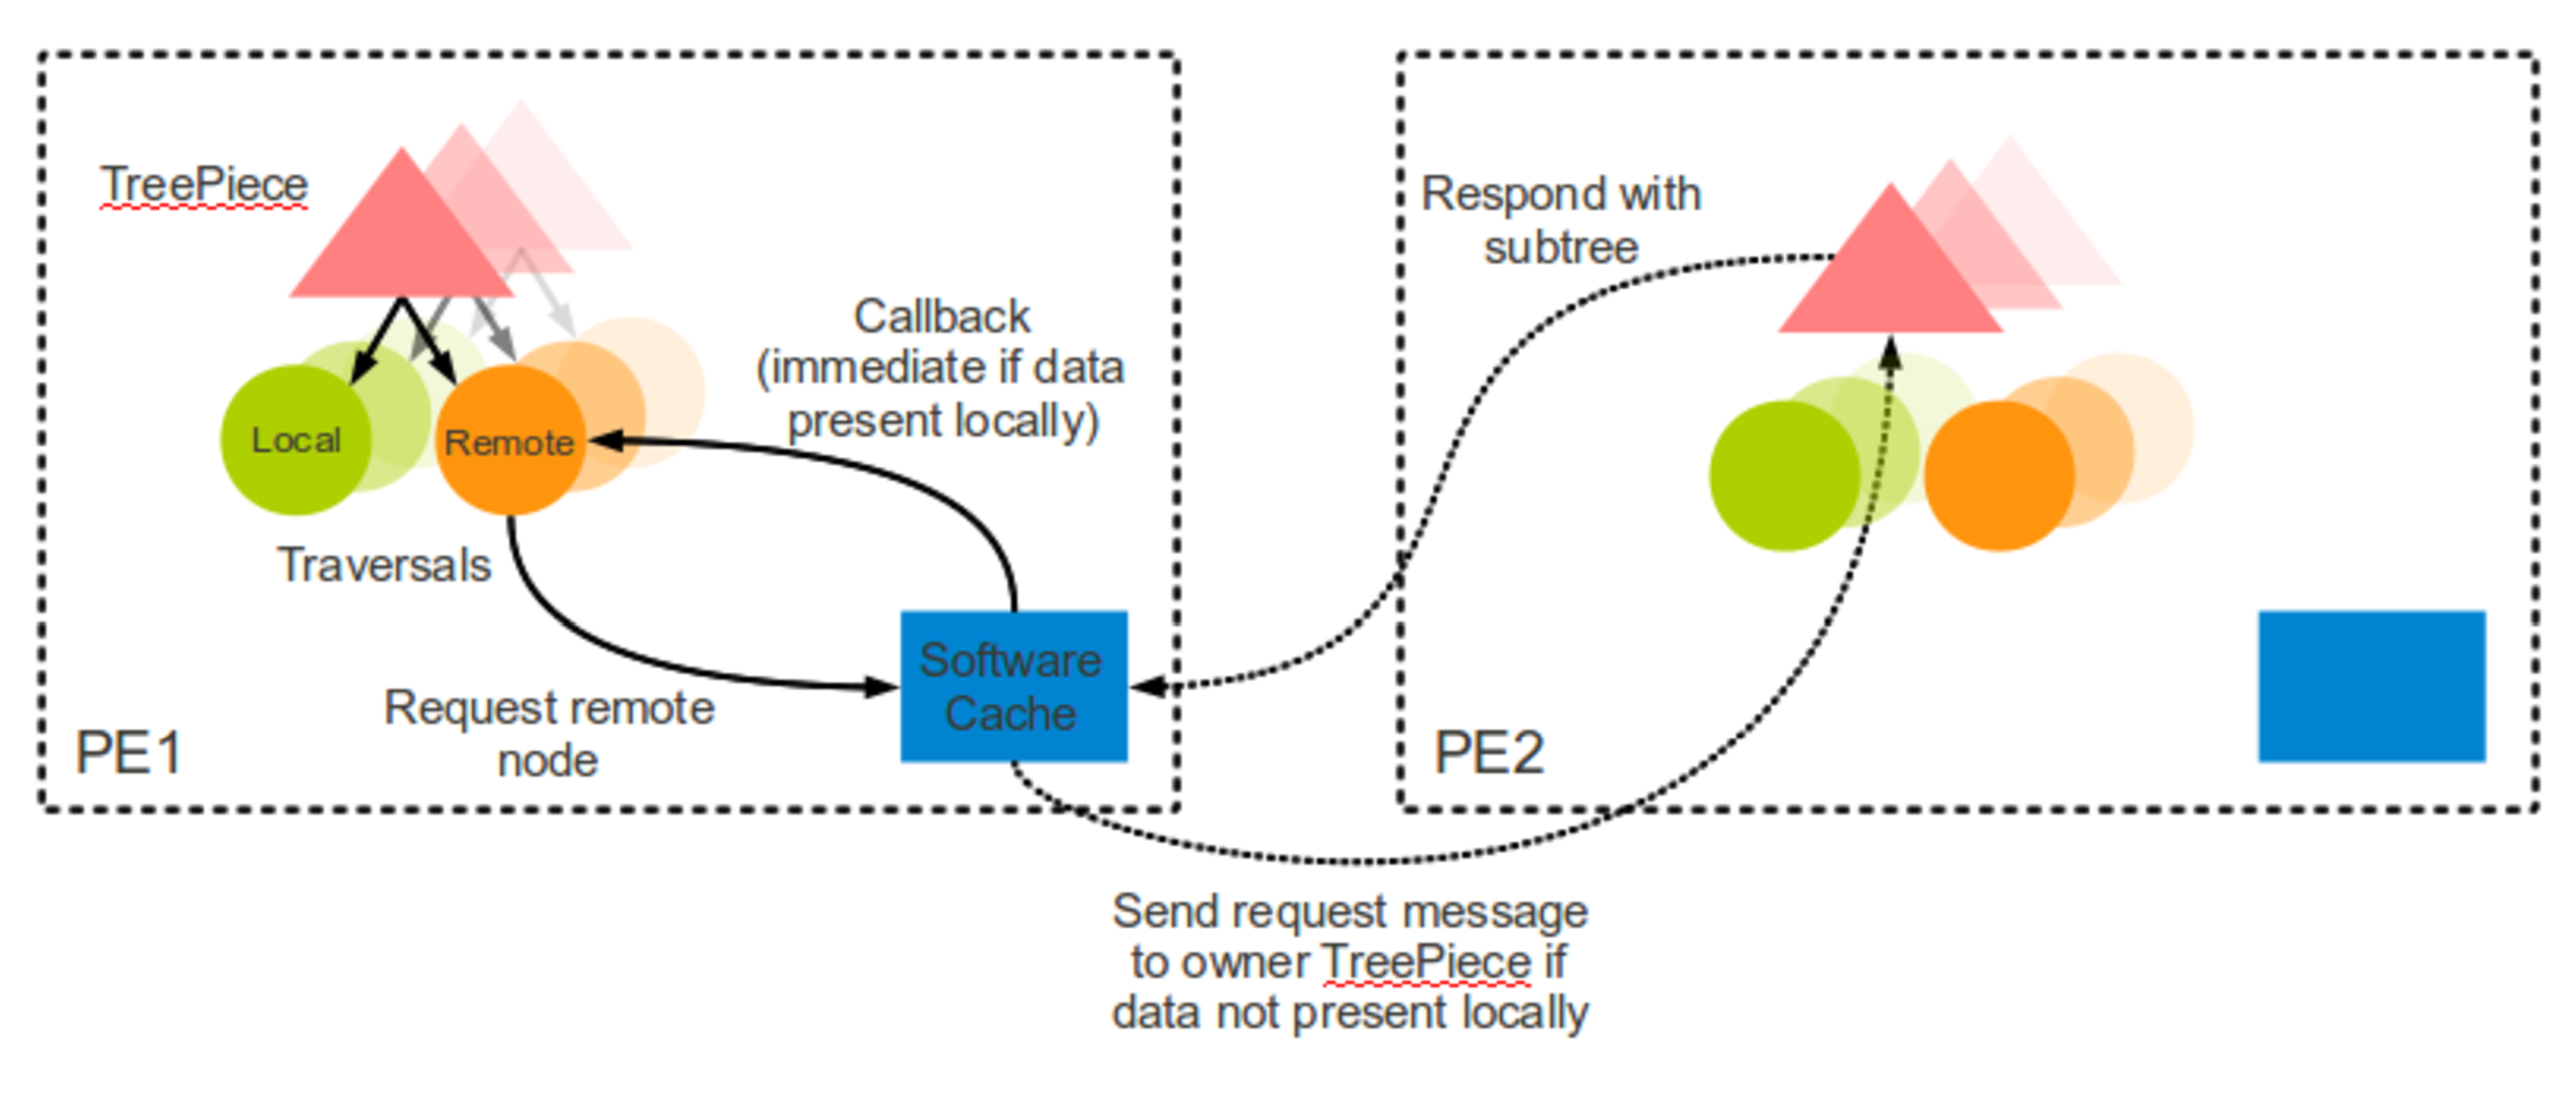
\includegraphics[width=\textwidth]{figures/changa.pdf} \end{center}
\end{frame}
